% This file is generated by the MATLAB m-file laprint.m. It can be included
% into LaTeX documents using the packages graphicx, color and psfrag.
% It is accompanied by a postscript file. A sample LaTeX file is:
%    \documentclass{article}\usepackage{graphicx,color,psfrag}
%    \begin{document}% This file is generated by the MATLAB m-file laprint.m. It can be included
% into LaTeX documents using the packages graphicx, color and psfrag.
% It is accompanied by a postscript file. A sample LaTeX file is:
%    \documentclass{article}\usepackage{graphicx,color,psfrag}
%    \begin{document}% This file is generated by the MATLAB m-file laprint.m. It can be included
% into LaTeX documents using the packages graphicx, color and psfrag.
% It is accompanied by a postscript file. A sample LaTeX file is:
%    \documentclass{article}\usepackage{graphicx,color,psfrag}
%    \begin{document}% This file is generated by the MATLAB m-file laprint.m. It can be included
% into LaTeX documents using the packages graphicx, color and psfrag.
% It is accompanied by a postscript file. A sample LaTeX file is:
%    \documentclass{article}\usepackage{graphicx,color,psfrag}
%    \begin{document}\input{fig_Preg_est_time_fading}\end{document}
% See http://www.mathworks.de/matlabcentral/fileexchange/loadFile.do?objectId=4638
% for recent versions of laprint.m.
%
% created by:           LaPrint version 3.16 (13.9.2004)
% created on:           09-Jun-2016 14:16:07
% eps bounding box:     16 cm x 12 cm
% comment:              
%
%\begin{psfrags}%
%\psfragscanon%
%
% text strings:
\psfrag{s05}[b][b]{\fontsize{8.5}{12.75}\fontseries{m}\mathversion{normal}\fontshape{n}\selectfont \color[rgb]{0,0,0}\setlength{\tabcolsep}{0pt}\begin{tabular}{c}$\preg$ [dBm]\end{tabular}}%
\psfrag{s06}[t][t]{\fontsize{8.5}{12.75}\fontseries{m}\mathversion{normal}\fontshape{n}\selectfont \color[rgb]{0,0,0}\setlength{\tabcolsep}{0pt}\begin{tabular}{c}$\tau$ [ms]\end{tabular}}%
\psfrag{s10}[][]{\fontsize{10}{15}\fontseries{m}\mathversion{normal}\fontshape{n}\selectfont \color[rgb]{0,0,0}\setlength{\tabcolsep}{0pt}\begin{tabular}{c} \end{tabular}}%
\psfrag{s11}[][]{\fontsize{10}{15}\fontseries{m}\mathversion{normal}\fontshape{n}\selectfont \color[rgb]{0,0,0}\setlength{\tabcolsep}{0pt}\begin{tabular}{c} \end{tabular}}%
\psfrag{s12}[l][l]{\fontsize{8.5}{12.75}\fontseries{m}\mathversion{normal}\fontshape{n}\selectfont \color[rgb]{0,0,0}Simulated}%
\psfrag{s13}[l][l]{\fontsize{8.5}{12.75}\fontseries{m}\mathversion{normal}\fontshape{n}\selectfont \color[rgb]{0,0,0}IM}%
\psfrag{s14}[l][l]{\fontsize{8.5}{12.75}\fontseries{m}\mathversion{normal}\fontshape{n}\selectfont \color[rgb]{0,0,0}EM}%
\psfrag{s15}[l][l]{\fontsize{8.5}{12.75}\fontseries{m}\mathversion{normal}\fontshape{n}\selectfont \color[rgb]{0,0,0}Simulated}%
%
% axes font properties:
\fontsize{8.5}{12.75}\fontseries{m}\mathversion{normal}%
\fontshape{n}\selectfont%
%
% xticklabels:
\psfrag{x01}[t][t]{$10^{-2}$}%
\psfrag{x02}[t][t]{$10^{-1}$}%
\psfrag{x03}[t][t]{$10^{0}$}%
\psfrag{x04}[t][t]{$10^{1}$}%
%
% yticklabels:
\psfrag{v01}[r][r]{-14}%
\psfrag{v02}[r][r]{-13}%
\psfrag{v03}[r][r]{-12}%
%
% Figure:
%\resizebox{8cm}{!}{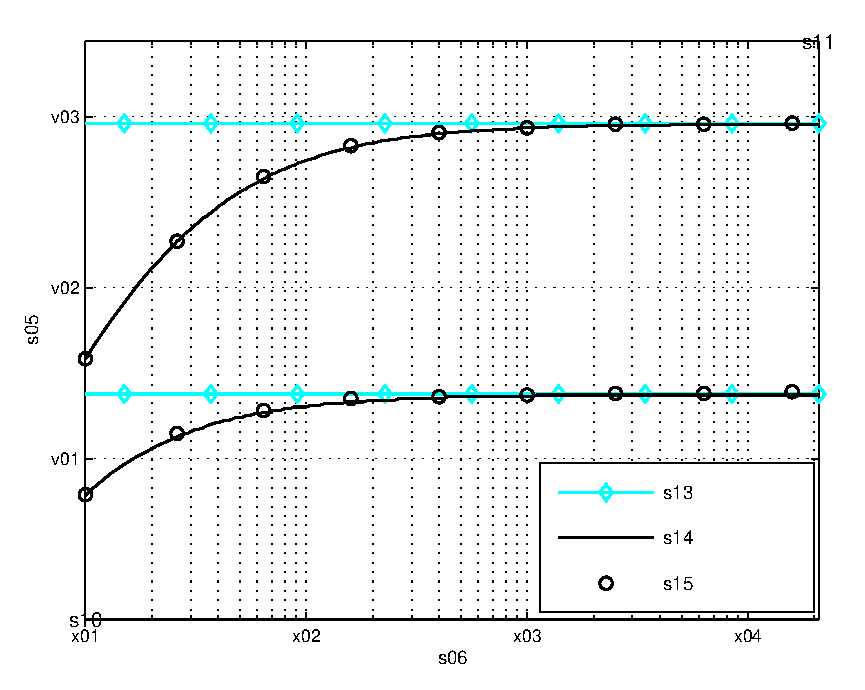
\includegraphics{fig_Preg_est_time_fading.eps}}%
%\end{psfrags}%
%
% End fig_Preg_est_time_fading.tex
\end{document}
% See http://www.mathworks.de/matlabcentral/fileexchange/loadFile.do?objectId=4638
% for recent versions of laprint.m.
%
% created by:           LaPrint version 3.16 (13.9.2004)
% created on:           09-Jun-2016 14:16:07
% eps bounding box:     16 cm x 12 cm
% comment:              
%
%\begin{psfrags}%
%\psfragscanon%
%
% text strings:
\psfrag{s05}[b][b]{\fontsize{8.5}{12.75}\fontseries{m}\mathversion{normal}\fontshape{n}\selectfont \color[rgb]{0,0,0}\setlength{\tabcolsep}{0pt}\begin{tabular}{c}$\preg$ [dBm]\end{tabular}}%
\psfrag{s06}[t][t]{\fontsize{8.5}{12.75}\fontseries{m}\mathversion{normal}\fontshape{n}\selectfont \color[rgb]{0,0,0}\setlength{\tabcolsep}{0pt}\begin{tabular}{c}$\tau$ [ms]\end{tabular}}%
\psfrag{s10}[][]{\fontsize{10}{15}\fontseries{m}\mathversion{normal}\fontshape{n}\selectfont \color[rgb]{0,0,0}\setlength{\tabcolsep}{0pt}\begin{tabular}{c} \end{tabular}}%
\psfrag{s11}[][]{\fontsize{10}{15}\fontseries{m}\mathversion{normal}\fontshape{n}\selectfont \color[rgb]{0,0,0}\setlength{\tabcolsep}{0pt}\begin{tabular}{c} \end{tabular}}%
\psfrag{s12}[l][l]{\fontsize{8.5}{12.75}\fontseries{m}\mathversion{normal}\fontshape{n}\selectfont \color[rgb]{0,0,0}Simulated}%
\psfrag{s13}[l][l]{\fontsize{8.5}{12.75}\fontseries{m}\mathversion{normal}\fontshape{n}\selectfont \color[rgb]{0,0,0}IM}%
\psfrag{s14}[l][l]{\fontsize{8.5}{12.75}\fontseries{m}\mathversion{normal}\fontshape{n}\selectfont \color[rgb]{0,0,0}EM}%
\psfrag{s15}[l][l]{\fontsize{8.5}{12.75}\fontseries{m}\mathversion{normal}\fontshape{n}\selectfont \color[rgb]{0,0,0}Simulated}%
%
% axes font properties:
\fontsize{8.5}{12.75}\fontseries{m}\mathversion{normal}%
\fontshape{n}\selectfont%
%
% xticklabels:
\psfrag{x01}[t][t]{$10^{-2}$}%
\psfrag{x02}[t][t]{$10^{-1}$}%
\psfrag{x03}[t][t]{$10^{0}$}%
\psfrag{x04}[t][t]{$10^{1}$}%
%
% yticklabels:
\psfrag{v01}[r][r]{-14}%
\psfrag{v02}[r][r]{-13}%
\psfrag{v03}[r][r]{-12}%
%
% Figure:
%\resizebox{8cm}{!}{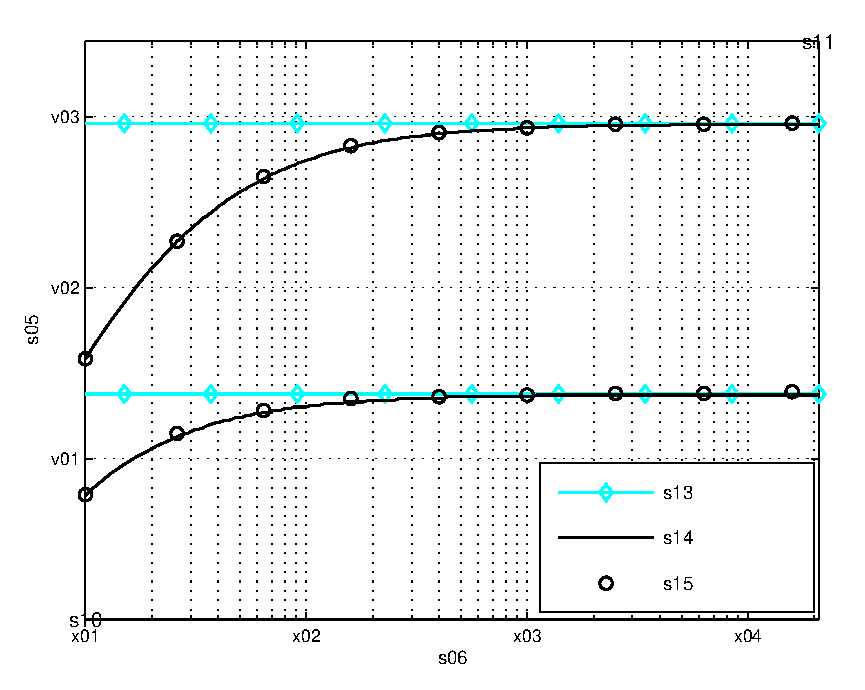
\includegraphics{fig_Preg_est_time_fading.eps}}%
%\end{psfrags}%
%
% End fig_Preg_est_time_fading.tex
\end{document}
% See http://www.mathworks.de/matlabcentral/fileexchange/loadFile.do?objectId=4638
% for recent versions of laprint.m.
%
% created by:           LaPrint version 3.16 (13.9.2004)
% created on:           09-Jun-2016 14:16:07
% eps bounding box:     16 cm x 12 cm
% comment:              
%
%\begin{psfrags}%
%\psfragscanon%
%
% text strings:
\psfrag{s05}[b][b]{\fontsize{8.5}{12.75}\fontseries{m}\mathversion{normal}\fontshape{n}\selectfont \color[rgb]{0,0,0}\setlength{\tabcolsep}{0pt}\begin{tabular}{c}$\preg$ [dBm]\end{tabular}}%
\psfrag{s06}[t][t]{\fontsize{8.5}{12.75}\fontseries{m}\mathversion{normal}\fontshape{n}\selectfont \color[rgb]{0,0,0}\setlength{\tabcolsep}{0pt}\begin{tabular}{c}$\tau$ [ms]\end{tabular}}%
\psfrag{s10}[][]{\fontsize{10}{15}\fontseries{m}\mathversion{normal}\fontshape{n}\selectfont \color[rgb]{0,0,0}\setlength{\tabcolsep}{0pt}\begin{tabular}{c} \end{tabular}}%
\psfrag{s11}[][]{\fontsize{10}{15}\fontseries{m}\mathversion{normal}\fontshape{n}\selectfont \color[rgb]{0,0,0}\setlength{\tabcolsep}{0pt}\begin{tabular}{c} \end{tabular}}%
\psfrag{s12}[l][l]{\fontsize{8.5}{12.75}\fontseries{m}\mathversion{normal}\fontshape{n}\selectfont \color[rgb]{0,0,0}Simulated}%
\psfrag{s13}[l][l]{\fontsize{8.5}{12.75}\fontseries{m}\mathversion{normal}\fontshape{n}\selectfont \color[rgb]{0,0,0}IM}%
\psfrag{s14}[l][l]{\fontsize{8.5}{12.75}\fontseries{m}\mathversion{normal}\fontshape{n}\selectfont \color[rgb]{0,0,0}EM}%
\psfrag{s15}[l][l]{\fontsize{8.5}{12.75}\fontseries{m}\mathversion{normal}\fontshape{n}\selectfont \color[rgb]{0,0,0}Simulated}%
%
% axes font properties:
\fontsize{8.5}{12.75}\fontseries{m}\mathversion{normal}%
\fontshape{n}\selectfont%
%
% xticklabels:
\psfrag{x01}[t][t]{$10^{-2}$}%
\psfrag{x02}[t][t]{$10^{-1}$}%
\psfrag{x03}[t][t]{$10^{0}$}%
\psfrag{x04}[t][t]{$10^{1}$}%
%
% yticklabels:
\psfrag{v01}[r][r]{-14}%
\psfrag{v02}[r][r]{-13}%
\psfrag{v03}[r][r]{-12}%
%
% Figure:
%\resizebox{8cm}{!}{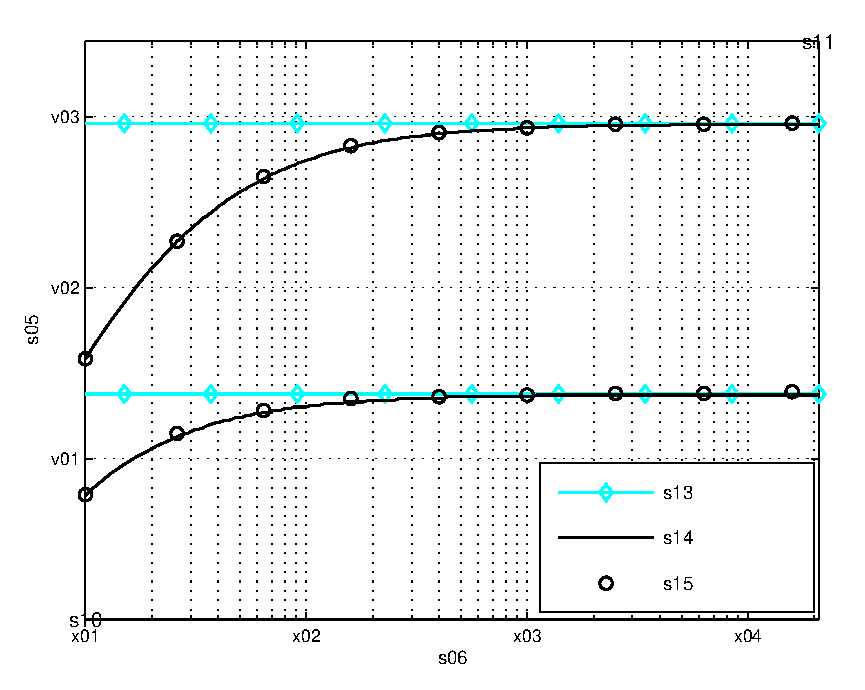
\includegraphics{fig_Preg_est_time_fading.eps}}%
%\end{psfrags}%
%
% End fig_Preg_est_time_fading.tex
\end{document}
% See http://www.mathworks.de/matlabcentral/fileexchange/loadFile.do?objectId=4638
% for recent versions of laprint.m.
%
% created by:           LaPrint version 3.16 (13.9.2004)
% created on:           09-Jun-2016 14:16:07
% eps bounding box:     16 cm x 12 cm
% comment:              
%
%\begin{psfrags}%
%\psfragscanon%
%
% text strings:
\psfrag{s05}[b][b]{\fontsize{8.5}{12.75}\fontseries{m}\mathversion{normal}\fontshape{n}\selectfont \color[rgb]{0,0,0}\setlength{\tabcolsep}{0pt}\begin{tabular}{c}$\preg$ [dBm]\end{tabular}}%
\psfrag{s06}[t][t]{\fontsize{8.5}{12.75}\fontseries{m}\mathversion{normal}\fontshape{n}\selectfont \color[rgb]{0,0,0}\setlength{\tabcolsep}{0pt}\begin{tabular}{c}$\tau$ [ms]\end{tabular}}%
\psfrag{s10}[][]{\fontsize{10}{15}\fontseries{m}\mathversion{normal}\fontshape{n}\selectfont \color[rgb]{0,0,0}\setlength{\tabcolsep}{0pt}\begin{tabular}{c} \end{tabular}}%
\psfrag{s11}[][]{\fontsize{10}{15}\fontseries{m}\mathversion{normal}\fontshape{n}\selectfont \color[rgb]{0,0,0}\setlength{\tabcolsep}{0pt}\begin{tabular}{c} \end{tabular}}%
\psfrag{s12}[l][l]{\fontsize{8.5}{12.75}\fontseries{m}\mathversion{normal}\fontshape{n}\selectfont \color[rgb]{0,0,0}Simulated}%
\psfrag{s13}[l][l]{\fontsize{8.5}{12.75}\fontseries{m}\mathversion{normal}\fontshape{n}\selectfont \color[rgb]{0,0,0}IM}%
\psfrag{s14}[l][l]{\fontsize{8.5}{12.75}\fontseries{m}\mathversion{normal}\fontshape{n}\selectfont \color[rgb]{0,0,0}EM}%
\psfrag{s15}[l][l]{\fontsize{8.5}{12.75}\fontseries{m}\mathversion{normal}\fontshape{n}\selectfont \color[rgb]{0,0,0}Simulated}%
%
% axes font properties:
\fontsize{8.5}{12.75}\fontseries{m}\mathversion{normal}%
\fontshape{n}\selectfont%
%
% xticklabels:
\psfrag{x01}[t][t]{$10^{-2}$}%
\psfrag{x02}[t][t]{$10^{-1}$}%
\psfrag{x03}[t][t]{$10^{0}$}%
\psfrag{x04}[t][t]{$10^{1}$}%
%
% yticklabels:
\psfrag{v01}[r][r]{-14}%
\psfrag{v02}[r][r]{-13}%
\psfrag{v03}[r][r]{-12}%
%
% Figure:
%\resizebox{8cm}{!}{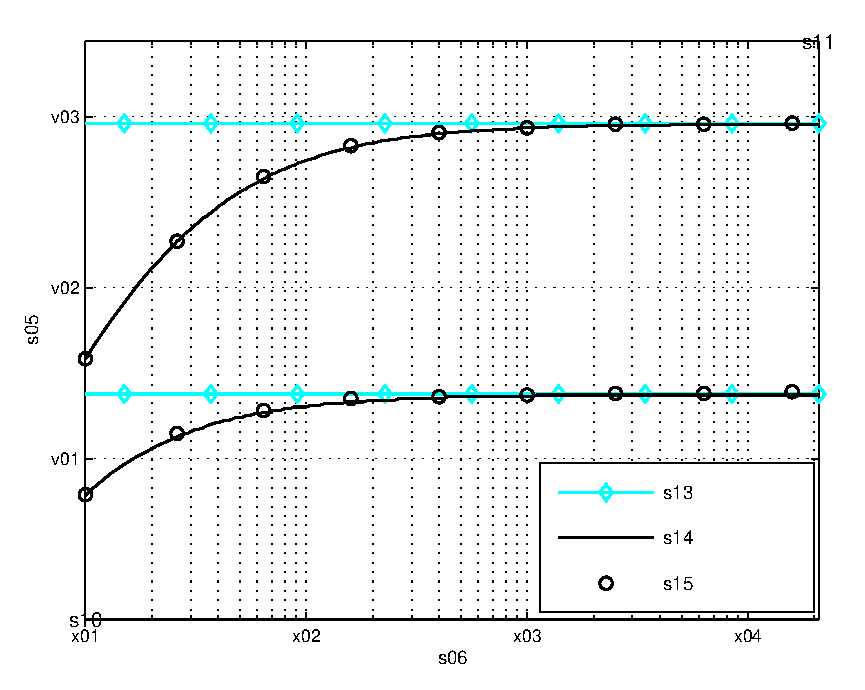
\includegraphics{fig_Preg_est_time_fading.eps}}%
%\end{psfrags}%
%
% End fig_Preg_est_time_fading.tex
